%!TEX root = ../thesis.tex
%*******************************************************************************
%****************************** Second Chapter *********************************
%*******************************************************************************

\chapter{Absorbtion of photon by an atom}  %Title of the Second Chapter
The purpose of this section is to outline the basic features observed in saturated absorption
spectroscopy and relate them to simple atomic and laser physics principles.
For this we will follow the guidance of \citep{SAS}.

\ifpdf{}
    \graphicspath{{Chapter2/Figs/Raster/}{Chapter2/Figs/PDF/}{Chapter2/Figs/}}
\else
    \graphicspath{{Chapter2/Figs/Vector/}{Chapter2/Figs/}}
\fi



%********************************** % First Section  *************************************
\section{Laser interactions~-~Two-level atom} %Section - 2.1

We begin with the interaction between a laser field and a sample of stationary atoms having
only two possible energy levels. Aspects of thermal motion will be treated subsequently.\\
The difference \(\Delta E = E_1 - E_0\) between the excited state \ket{e} energy \(E_1\) and
ground state \ket{g} energy \(E_0\) is used with Planck's law to determine the photon frequency
\(\nu \) associated with transitions between the two states:
\begin{align}
    \Delta E = h \nu_0
\end{align}
There are three transition processes involving atoms and laser fields:
\bigskip

\begin{minipage}[c][][c]{.35\textwidth}
\begin{itemize}
\item[(1)] stimulated absorption
\item[(2)] stimulated emission
\item[(3)] spontaneous emission
\end{itemize}
\end{minipage}
\hfill
\begin{minipage}[c]{.55\textwidth}
\includegraphics[width=\textwidth]{twolevel}
\captionof{figure}{Two-level atom model}
\end{minipage}
\bigskip

We consider spontaneous emission first~--~a process characterized by a transition rate or probability
per unit time for an atom in the excited state to decay to the ground state. This transition rate will 
be denoted \(\Gamma_\omega \) and is about \(2\pi\cdot \SI{1.3}{\mega\hertz} \) for the rubidium levels
studied here. \\
In the absence of an external field, any initial population of excited state atoms would decay exponentially
to the ground state with a mean life time \(\Delta t = 1/\Gamma_\omega \approx \SI{122}{\nano\second} \).
In the rest frame of the atom, spontaneous photons are emitted in all directions with an energy spectrum
having a mean \(E=h\nu_0 \) and a full width at half maximum (FWHM) \(\Delta E \) given by the
Heisenberg uncertainty principle \(\Delta E \Delta t = \hbar \) or \(\Delta E = \Gamma_\omega\hbar \).
Experssed in frequency units, the FWHM is called the \textit{natural linewidth} and given the symbol
\(\Gamma_\nu \). Thus
\begin{align}
    \Gamma_\nu = \frac{\Gamma_\omega}{2\pi}
\end{align}
For our rubidium levels, \(\Delta E \approx 5.4\cdot \SI{e-9}{\electronvolt} \) or \(\Gamma_\nu\approx \SI{1.3}{\mega\hertz} \). \\ 
The stimulated emission and absorption processes are also described by a transition rate~--~a single rate
giving the probability per unit time for a ground state atom to absorb a laser photon or for an excited
state atom to emit a laser photon. The stimulated transition rate is proportional to the laser intensity
\textit{I} (SI units of \si{\watt\per\meter\squared}) and is only significantly different from zero when
the laser frequency \(\nu \) is near the resonance frequency \(\nu_0 \). This transition rate will be denoted
\(\alpha I \), where 

\begin{minipage}[c][][c]{.45\textwidth}
\begin{align}
    \alpha = \alpha_0 \mathl{L}(\nu,\nu_0)
\end{align}
and
\begin{align}
    \mathl{L}(\nu,\nu_0) &= \frac{1}{ 1+4 {(\nu-\nu_0)}^2 / {\Gamma_\nu}^2 }
\end{align}
\end{minipage}
\hfill
\begin{minipage}[c]{.45\textwidth}
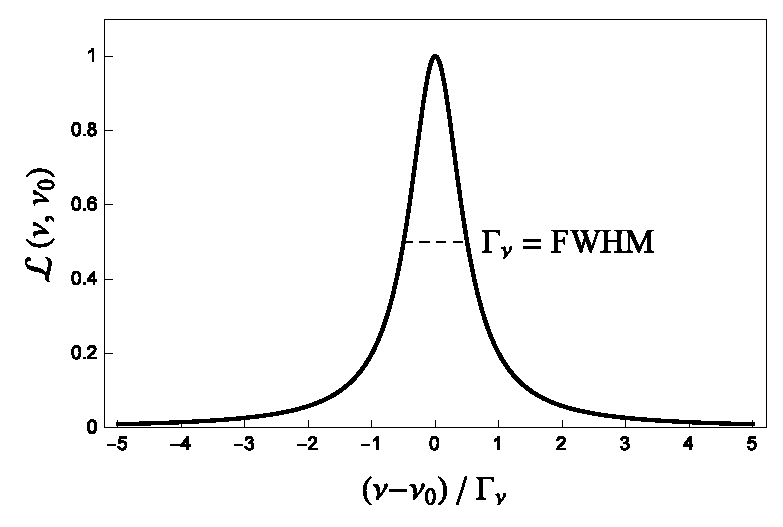
\includegraphics[width=\textwidth]{nLinewidth}
\captionof{figure}{The Lorentzian line shape profile for resonance absorption}
\label{fig:nlinewidth}
\end{minipage}
\bigskip

gives the \textit{Lorentzian} frequency dependence as shown in Fig.~\ref{fig:nlinewidth}.
\(\mathl{L}(\nu,\nu_0) \) also describes the spectrum of radiation from spontaneous emission
and the width \(\Gamma_\nu \) is the same for both cases. The maximum transition rate 
\(\alpha_0 I \) occors right on resonance (\(\nu~=~\nu_0 \)).\\
The value of \(\Gamma_\omega / \alpha_0 \) defines the saturation intensity \(I_{sat} \) of the
atoms. Its significance is that when the laser intensity is equal to the saturation intensity,
excited state atoms are equally likely to decay by stimulated emission or by spontaneous emission.
\pagebreak

%********************************** % Second Section  *************************************
\section{Basic laser absorption spectroscopy}   %Section - 2.2



\begin{align}
    I(x+\mathrm{d}x)-I(x) = - I(x) h\nu \alpha n  (P_0-P_1) \mathrm{d}x \label{int_eq}
\end{align}

where:
\begin{itemize}
    \setlength{\itemsep}{0ex}
    \item[\(\alpha I(x)\)]\ldots~stimulated transition rate
    \item[n]\ldots~atom density
    \item[\(P_0\)]\ldots~proportion of atoms in \ket{g}
    \item[\(P_1\)]\ldots~proportion of atoms in \ket{e}
\end{itemize}
\pagebreak
%********************************** % Fourth Section  *************************************
\section{Absorption coefficient}  %Section - 1.4
Out of equation~(\ref{int_eq}) we define the absorption coefficient \(\kappa \):
\begin{align}
    \kappa = h\nu \alpha n  (P_0-P_1) \label{kappa}
\end{align}
With the next steps we wanna decribe the different parameters and derive \(\kappa \) with all
its dependencies. For this we will follow the guidance of \citep{SAS}.
\bigskip

\(h\nu \) is the excitation energy for the atom to change from ground \ket{g} to excited state \ket{e}. \\
From the stimulated transition rate \(\alpha \) denotes:
\begin{align}
    \alpha = \alpha_0 \mathl{L}(\nu,\nu_0)
\end{align}
where
\begin{align}
    \alpha_0 &= \frac{2\pi\Gamma}{I_{sat}} \\
    \mathl{L}(\nu,\nu_0) &= \frac{1}{ 1+\frac{ 4{(\nu-\nu_0)}^2 }{\Gamma^2} }
\end{align}

%\begin{figure}[h]
%\centering
%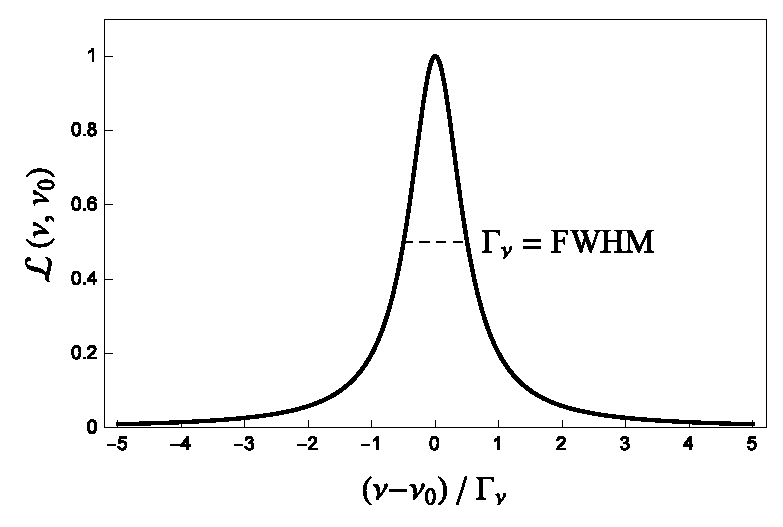
\includegraphics[width=0.6\textwidth]{nLinewidth}
%\caption{The Lorentzian line shape profile for resonance absorption}
%\label{fig:nlinewidth} 
%\end{figure}

\pagebreak
%********************************** % Fifth Section  *************************************
\section{Doppler shifts}  %Section - 1.5

\pagebreak
%********************************** % Sixth Section  *************************************
\section{Behavior of absorption coefficient}  %Section - 1.6

\pagebreak
%********************************** % Seventh Section  *************************************
\section{Non-linear differential equation}  %Section - 1.7

\pagebreak

\section{Relevant data}

\begin{table}[h]
\centering
\begin{tabular*}{0.5\textwidth}{@{\extracolsep{\fill} }l c c}
\toprule
& \multicolumn{2}{c}{Rubidium} \\
\midrule
Isotope & 85 & 87 \\
Atomic mass & 84.911794 & 86.909187 \\
in \(10^{-25}\)kg & 1.40999 & 1.44316 \\
Abundance & 72.17\% & 27.83\% \\
Spin I & \(\sfrac{5}{2}\) & \(\sfrac{3}{2}\) \\
lifetime \(6^{2}P_{3/2}\) & \multicolumn{2}{c}{\SI{112}{\nano\second}} \\
Natural linewidth & \multicolumn{2}{c}{\(2\pi \times \SI{1.421}{\mega\hertz}\) } \\
\bottomrule
\end{tabular*}
\caption{Properties of rubidium isotopes}
\label{table:iso_prop}
\end{table}
\pagebreak

%********************************** % Eighth Section  *************************************

\section{D2 line} %Section - 1.2 

\begin{figure}[h]
\centering
\includegraphics[width=0.9\textwidth]{energylevel}
\caption{\(5^{2}S_{1/2} \rightarrow 6^{2}P_{3/2}\) transition of \(^{85}\)Rb and \(^{87}\)Rb with corresponding hyperfine structure}    
\end{figure}

\vspace{\fill}

The transition of interest is, as we have discussed before, the \(5^{2}S_{1/2} \rightarrow 6^{2}P_{3/2}\) of rubidium. As known rubidium
occurs in two isotopes, \(^{85}\)Rb and \(^{87}\)Rb.
As we can see both isotopes have the same transition energy, but due to the different spin I (see table:~\ref{table:iso_prop}) we get
different energy levels for the groundstate \citep{nist_asd}. This is the reason why we wittness four doppler peaks in our spectrum.
\bigskip

\textbf{Caution:} Both figures below show the correct correlation between energy and isotopes. The reason for this is that the spectrum
shows transition energy and the other one the specific energy levels.

\vspace{\fill}

\begin{figure}[h]
\centering
\includegraphics[width=0.6\textwidth]{spectrum_doppler}
\caption{Doppler spectrum of D2 line}
\label{fig:doppler} 
\end{figure}

\vspace{\fill}

\begin{figure}[h]
\centering
\includegraphics[width=0.6\textwidth]{groundstate}
\caption{Relative energy gaps of the groundstates between both isotopes}
\label{fig:gap} 
\end{figure}